\documentclass[aspectratio=169,10pt]{beamer}
\usetheme{Madrid}
\usecolortheme{default}
\usepackage[T1]{fontenc}
\usepackage{lmodern}
\usepackage{tikz}
\usepackage{booktabs}
\usepackage{fontawesome5}
\usepackage{xcolor}
\usepackage{mathtools}
\usepackage{colortbl}
\usepackage{multirow}
\usepackage{bbm}
\usepackage{listings}
\usepackage{bookmark}
\usepackage{amsmath}    % Essential for many math features
\usepackage{amsfonts}   % Provides \mathbb
\usepackage{amssymb}
\usepackage[most]{tcolorbox}
\usepackage[backend=biber, style=numeric, sorting=none, maxnames=3, minnames=1]{biblatex}
\addbibresource{references.bib}
\usetikzlibrary{arrows.meta,shadows,positioning,fit,shapes.geometric,calc, shadows.blur, backgrounds}

\lstdefinestyle{ccode}{
  language=C,
  basicstyle=\ttfamily\scriptsize,
  keywordstyle=\color{c1}\bfseries,
  commentstyle=\color{hit!80!black}\itshape,
  breaklines=true,
  showstringspaces=false,
  tabsize=2,
}
\setbeamertemplate{enumerate item}{\arabic{enumi}.}
\setbeamertemplate{itemize item}{--}
\setbeamertemplate{itemize subitem}{--}

% ── palette ──────────────────────────────────────────────────────────
\definecolor{c1}{RGB}{41,128,185}
\definecolor{c2}{RGB}{52,152,219}
\definecolor{c3}{RGB}{155,89,182}
\definecolor{c4}{RGB}{142,68,173}
\definecolor{c5}{RGB}{230,126,34}
\definecolor{c6}{RGB}{211,84,0}
% \definecolor{banana}{RGB}{253, 231, 76} 
% \definecolor{strongcyan}{RGB}{78, 205, 196}
% \definecolor{spaceindigo}{RGB}{195, 195, 230}
% \definecolor{powderblush}{RGB}{247, 177, 171}
\definecolor{c7}{RGB}{63,81,181}
\definecolor{c8}{RGB}{0,128,128}
\definecolor{c9}{RGB}{219,39,119}
\definecolor{hit}{RGB}{39,174,96}
\definecolor{miss}{RGB}{192,57,43}
\definecolor{warn}{RGB}{243,156,18}

\setbeamercolor{frametitle}{bg=c1,fg=white}
\setbeamercolor{title}{fg=white}
\setbeamercolor{structure}{fg=c1}
\setbeamertemplate{navigation symbols}{}
\setbeamertemplate{footline}[frame number]
\setbeamerfont{frametitle}{series=\bfseries}

\newcommand{\chit}[1]{\cellcolor{hit!30} #1}
\newcommand{\cmiss}[1]{\cellcolor{miss!25} #1}
\newcommand{\cwarn}[1]{\cellcolor{warn!30} #1}
\newcommand{\czero}{\cellcolor{black!4} }

\definecolor{slidebg}{RGB}{248, 250, 252}
\definecolor{trackoff}{RGB}{238, 242, 255}
\definecolor{trackon}{RGB}{236, 253, 245}
\definecolor{borderoff}{RGB}{99, 102, 241}
\definecolor{borderon}{RGB}{16, 185, 129}

% Node chips
\definecolor{ccode}{RGB}{239, 68,  68}
\definecolor{ccpg}{RGB}{59,  130, 246}
\definecolor{csub}{RGB}{16,  185, 129}
\definecolor{cemb}{RGB}{168, 85,  247}
\definecolor{ckb}{RGB}{245, 158, 11}
\definecolor{crank}{RGB}{236, 72,  153}

% Text / labels
\definecolor{labelcol}{RGB}{30,  41,  59}
\definecolor{notecol}{RGB}{100, 116, 139}
\definecolor{headcol}{RGB}{15,  23,  42}

% Shadow color
\definecolor{shadowcol}{RGB}{101, 67, 33}     % warm brown


\definecolor{cvecolor}{RGB}{231,76,60}
\definecolor{llmcolor}{RGB}{52,152,219}
\definecolor{snippetcolor}{RGB}{155,89,182}
\definecolor{augmentcolor}{RGB}{243,156,18}
\definecolor{trivialcolor}{RGB}{39,174,96}
\definecolor{nontrivialcolor}{RGB}{230,126,34}
\definecolor{finalcolor}{RGB}{44,62,80}

\setbeamercolor{background canvas}{bg=slidebg}
% \setbeamercolor{frametitle}{fg=headcol}
% \setbeamerfont{frametitle}{series=\bfseries, size=\large}


\title{CVEFixes experiments: Full Files as Input}
\subtitle{Checkpoint 8}
\author{Lívia Cavalcanti}
\date{July 2026}

% TODO: add supervisors names and affiliations if desired

\begin{document}

% =====================================================================
% TITLE SLIDE
% =====================================================================
\begin{frame}[plain]
  \titlepage
  
\end{frame}

\begin{frame}[fragile]{Evaluation Metrics}

  \begin{center}
  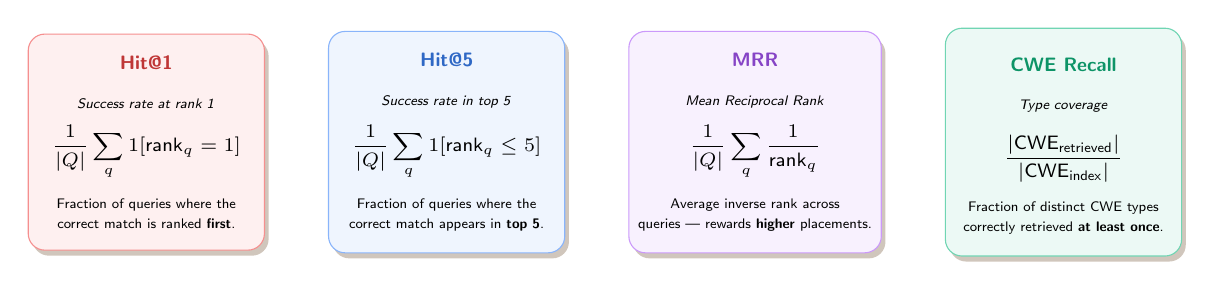
\begin{tikzpicture}[
    node distance=0.6cm and 1.2cm,
    mcard/.style={
      draw=#1!60, fill=#1!8,
      rounded corners=6pt,
      minimum width=3cm,
      minimum height=2.4cm,
      inner ysep=8pt,
      font=\scriptsize\sffamily,
      align=center,
      drop shadow={shadow xshift=1.5pt, shadow yshift=-2pt, opacity=0.3, fill=shadowcol}
    },
    mtitle/.style={
      font=\scriptsize\sffamily\bfseries,
      text=#1!80!black
    },
    micon/.style={
      font=\Large,
      text=#1
    }
  ]

    % --- Card 1: Hit@1 ---
    \node[mcard=ccode] (h1) {
      % \textcolor{ccode}{\faBuilding}\\[4pt]
      {\scriptsize\bfseries\textcolor{ccode!80!black}{Hit@1}}\\[6pt]
      {\tiny\textit{Success rate at rank 1}}\\[5pt]
      $\displaystyle\frac{1}{|Q|}\sum_{q} \mathbbm{1}[\text{rank}_q = 1]$\\[6pt]
      {\tiny Fraction of queries where the}\\[-1pt]
      {\tiny correct match is ranked \textbf{first}.}
    };

    % --- Card 2: Hit@5 ---
    \node[mcard=ccpg, right=0.8cm of h1] (h5) {
      % \textcolor{ccpg}{\faListOl}\\[4pt]
      {\scriptsize\bfseries\textcolor{ccpg!80!black}{Hit@5}}\\[6pt]
      {\tiny\textit{Success rate in top 5}}\\[5pt]
      $\displaystyle\frac{1}{|Q|}\sum_{q} \mathbbm{1}[\text{rank}_q \leq 5]$\\[6pt]
      {\tiny Fraction of queries where the}\\[-1pt]
      {\tiny correct match appears in \textbf{top 5}.}
    };

    % --- Card 3: MRR ---
    \node[mcard=cemb, right=0.8cm of h5] (mrr) {
      % \textcolor{cemb}{\faSortAmountDown}\\[4pt]
      {\scriptsize\bfseries\textcolor{cemb!80!black}{MRR}}\\[6pt]
      {\tiny\textit{Mean Reciprocal Rank}}\\[5pt]
      $\displaystyle\frac{1}{|Q|}\sum_{q} \frac{1}{\text{rank}_q}$\\[6pt]
      {\tiny Average inverse rank across}\\[-1pt]
      {\tiny queries — rewards \textbf{higher} placements.}
    };

    % --- Card 4: CWE Recall ---
    \node[mcard=csub, right=0.8cm of mrr] (cwe) {
      \\[-0.5pt]
      % \textcolor{csub}{\faProjectDiagram}\\[4pt]
      {\scriptsize\bfseries\textcolor{csub!80!black}{CWE Recall}}\\[6pt]
      {\tiny\textit{Type coverage}}\\[7pt]
      $\displaystyle\frac{|\text{CWE}_{\text{retrieved}}|}{|\text{CWE}_{\text{index}}|}$\\[6pt]
      {\tiny Fraction of distinct CWE types}\\[-1pt]
      {\tiny correctly retrieved \textbf{at least once}.}
      % \\[-0.01pt]
    };

  \end{tikzpicture}
  \end{center}
 

\end{frame}
% =====================================================================
% PHASE 1: AUTOPATCH RESULTS
% =====================================================================
\begin{frame}{ AutoPatch Dataset Results (n=225)}
  % \textbf{Goal:} Validate that structural embeddings match CodeBERT performance.

  \vspace{0.3cm}
  \begin{table}
    \centering
    \small
    \begin{tabular}{lrrrr}
      \toprule
      \textbf{Embedder} & \textbf{H@1} & \textbf{H@5} & \textbf{MRR} & \textbf{CWE R.} \\
      \midrule
      \multicolumn{5}{c}{\textit{Structure-Only}} \\
      \midrule
      \textbf{Combined} & \textbf{0.8904} & \textbf{0.9589} & \textbf{0.9162} & \textbf{0.4978} \\
      GIN & 0.7260 & 0.8767 & 0.7879 & 0.4427 \\
      WL & 0.6986 & 0.7945 & 0.7363 & 0.4386 \\
      \midrule
      \multicolumn{5}{c}{\textit{CodeBERT pretrained}} \\
      \midrule
      CodeBERT (baseline) & 0.1533 & 0.2200 & 0.1826 & 0.2933 \\
      CodeBERT (seq) & 0.7534 & 0.8630 & 0.7927 & 0.4121 \\
CodeBERT (pat) & 0.7123 & 0.8356 & 0.7677 & 0.4147 \\      \bottomrule
    \end{tabular}
    \\[2pt]
    {\tiny\textcolor{notecol}{Source: \texttt{experiments/output/checkpoint5/20260505\_141347\_experiment\_f59ab1/results.json}}}
  \end{table}

  
  \textbf{RQ1:} validated — structural \textit{graph} representations are \textit{effective} for vulnerability pattern retrieval in a synthetic dataset.
\end{frame}



% =====================================================================
% PHASE 2: CVEFIXES RESULTS
% =====================================================================
\begin{frame}{Motivation: Function vs.\ File Input}

  \textbf{Goal:} compare CVEfixes retrieval when each CPG is built from the
  \textcolor{miss!80!black}{\textbf{function}} field vs.\ the full
  \textcolor{hit!70!black}{\textbf{file}} field.

  \vspace{0.5em}
  \begin{columns}[T]
    % ---- Function input: malformed CPG ----
    \begin{column}{0.5\textwidth}
      \begin{center}
        {\small\textbf{\textcolor{miss}{Function input}}}\\[1pt]
        {\tiny\color{notecol} malformed CPG}\\[8pt]
        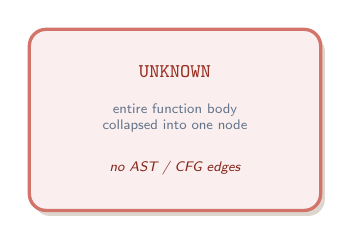
\begin{tikzpicture}[every node/.style={font=\scriptsize\sffamily}]
          \node[draw=miss!70, fill=miss!8, rounded corners=6pt, very thick,
                minimum width=3.7cm, minimum height=2.3cm, align=center,
                drop shadow={shadow xshift=1.5pt, shadow yshift=-2pt,
                             opacity=0.22, fill=shadowcol}]
            {%
              {\ttfamily\bfseries\color{miss!80!black} UNKNOWN}\\[5pt]
              {\tiny\color{notecol} entire function body}\\[-2pt]
              {\tiny\color{notecol} collapsed into one node}\\[7pt]
              {\tiny\itshape\color{miss!70!black} no AST / CFG edges}%
            };
        \end{tikzpicture}\\[6pt]
        {\tiny\color{notecol} 1 node \;$\cdot$\; label \texttt{UNKNOWN} \;$\cdot$\; 0 edges}
      \end{center}
    \end{column}
    % ---- File input: well-formed CPG ----
    \begin{column}{0.5\textwidth}
      \begin{center}
        {\small\textbf{\textcolor{hit!70!black}{File input}}}\\[1pt]
        {\tiny\color{notecol} well-formed CPG}\\[8pt]
        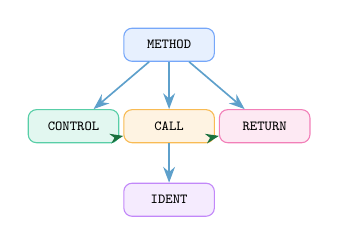
\begin{tikzpicture}[
            >=Stealth,
            nd/.style={rounded corners=3pt, font=\tiny\ttfamily,
                       minimum width=1.15cm, minimum height=0.42cm, align=center},
            ast/.style={->, draw=c1!75, semithick},
            cfg/.style={->, draw=hit!65!black, dashed}
          ]
          \node[nd, draw=ccpg!70,  fill=ccpg!12]                                    (m)    {METHOD};
          \node[nd, draw=csub!70,  fill=csub!12,  below left=0.6cm and 0.05cm of m]  (ctl)  {CONTROL};
          \node[nd, draw=ckb!70,   fill=ckb!12,   below=0.6cm of m]                  (call) {CALL};
          \node[nd, draw=crank!70, fill=crank!12, below right=0.6cm and 0.05cm of m] (ret)  {RETURN};
          \node[nd, draw=cemb!70,  fill=cemb!12,  below=0.5cm of call]               (id)   {IDENT};
          \draw[ast] (m) -- (ctl);
          \draw[ast] (m) -- (call);
          \draw[ast] (m) -- (ret);
          \draw[ast] (call) -- (id);
          \draw[cfg] (ctl)  to[bend right=12] (call);
          \draw[cfg] (call) to[bend right=12] (ret);
        \end{tikzpicture}\\[6pt]
        {\tiny\color{notecol} typed nodes \;$\cdot$\; \textcolor{c1}{solid AST} \,/\, \textcolor{hit!65!black}{dashed CFG}}
      \end{center}
    \end{column}
  \end{columns}

  \vspace{0.4em}
  \begin{tcolorbox}[colback=warn!6, colframe=warn!70!black, boxrule=0.35pt,
    left=4pt, right=4pt, top=2pt, bottom=2pt, arc=2pt, width=\linewidth]
    \scriptsize
    \textbf{Why:} inspecting the function-field graphs revealed they were frequently
    \textbf{not well-formed} --- Joern collapsed the whole body into a
    \textbf{single node labeled \texttt{UNKNOWN}}, erasing the AST / CFG structure the
    embedders depend on. Rebuilding each CPG from the \textbf{full file} restores proper
    node typing and control/data-flow edges, motivating the comparison that follows.
  \end{tcolorbox}

\end{frame}


\begin{frame}{CVEfixes Dataset }
  
  \textbf{Question:} Does the approach generalize to real-world vulnerabilities?
  \vspace{0.3cm}
  
\begin{columns}[T]
\begin{column}{0.48\textwidth}

  \textbf{Real-World Dataset}\\[3pt]
  {\small CVEFixes \cite{bhandari2021cvefixes} datasets is large dataset with real-world CVEs collected from the U.S. National Vulnerability Database, patches, and code changes.\\}
  
  \vspace{0.5em}
  \begin{center}
    
  \scriptsize
  \begin{tabular}{lr}
    \toprule
    \textbf{Metric} & \textbf{Value} \\
    \midrule
    CVEs & 11,873 \\
    Fix commits & 12,107 \\
    File changes & 51,342 \\
    Method changes & 277,948 \\
    Repositories & 4,249 \\
    \bottomrule
  \end{tabular}
  \end{center}
\end{column}
\begin{column}{0.50\textwidth}
    {\small\textbf{Sampling criteria}}\\[3pt]
  {\scriptsize
  \begin{itemize}\itemsep1pt
      \setbeamertemplate{itemize item}{}
    \item Structurally distinshable CWEs (e.g. UAF vs. OOB) to test pattern matching, not just code similarity
    \item Balanced superclass(CWE) up to 20 entries and subclasses (CVE) to ensure retrieval feasibility
  \end{itemize}}
      \vspace{0.5em}
    \begin{center}

  {\scriptsize
  \renewcommand{\arraystretch}{1.2}
  \begin{tabular}{lr}
    \toprule
    \textbf{Parameter} & \textbf{Value} \\
    \midrule
    Total pairs & 136 \\
    Index set & 109 \\
    Query set & 27 \\
    Unique CVEs (index) & 60 \\
    Unique CVEs (query) & 25 \\
    CWE classes & 7 \\
    % Slice depth & 2-hop \\
    % Min/max lines & 10 / 120 \\
    \bottomrule
  \end{tabular}}

    \end{center}
  
\end{column}
\end{columns}
\end{frame}


\begin{frame}{Balanced Dataset + Function Graph Input: Retrieval Results}

  \begin{columns}[T]
    \begin{column}{0.5\textwidth}

  \begin{center}
    {\small\textbf{Same-CWE Retrieval} {\scriptsize(n=109 index, 27 query)}}\\[6pt]
  {\scriptsize
  \renewcommand{\arraystretch}{1.35}
  \setlength{\tabcolsep}{3.5pt}
    \begin{tabular}{lrrrr}
      \toprule
      \textbf{Embedder} & \textbf{Hit@1} & \textbf{Hit@5} & \textbf{MRR} & \textbf{CWE Recall} \\
      \midrule
      GIN & 0.259 & 0.778 & 0.315 & 0.202 \\
      \rowcolor{warn!12}
      Combined & \cmiss{0.111} & 0.778 & 0.223 & 0.189 \\
      CodeBERT (baseline) & 0.080 & 0.1518 & 0.098 & 0.141 \\
      \rowcolor{hit!12}
      \textbf{CodeBERT (seq)} & \textbf{0.556} & \textbf{0.926} & \textbf{0.555} & \textbf{0.264} \\
      \textbf{CodeBERT (pat)} & \textbf{0.519} & \textbf{0.889} & \textbf{0.549} & \textbf{0.276} \\
      \bottomrule
    \end{tabular}
  }

  \vspace{0.3em}
  {\tiny\textcolor{notecol}{Source: \texttt{cvefixes\_experiments/output/pipeline\_verification/results.json}}}

  
  \end{center}
  
    \end{column}
    \begin{column}{0.5\textwidth}

  \begin{center}
  {\small\textbf{Per-CWE Breakdown} {\scriptsize(CodeBERT Pattern, CWE Hit@$k$)}}\\[6pt]
  {\scriptsize
  \renewcommand{\arraystretch}{1.35}
  \setlength{\tabcolsep}{3.5pt}
  \begin{tabular}{l r rrr}
    \toprule
    \textbf{CWE} & \textbf{N} & \textbf{Hit@1} & \textbf{Hit@5} & \textbf{Hit@10} \\
    \midrule
    Integer Overflow (190) & 4 & \chit{75\%} & 100\% & 100\% \\
    Input Validation (20) & 4 & \chit{75\%} & 75\% & 100\% \\
    Resource Consump.\ (400) & 3 & \chit{67\%} & 100\% & 100\% \\
    Use After Free (416) & 4 & 50\% & 100\% & 100\% \\
    NULL Ptr Deref (476) & 5 & \cwarn{40\%} & 80\% & 80\% \\
    Race Condition (362) & 3 & \cwarn{33\%} & 100\% & 100\% \\
    OOB Write (787) & 4 & \cmiss{25\%} & 75\% & 75\% \\
    \midrule
    \textbf{Overall} & \textbf{27} & \textbf{51.9\%} & \textbf{88.9\%} & \textbf{92.6\%} \\
    \bottomrule
  \end{tabular}}

  \vspace{0.2em}
  {\tiny\textcolor{notecol}{Source: same file (CodeBERT Pattern cell)}}

  \vspace{0.2em}
  {\scriptsize\textcolor{notecol}{Highlights areas for improvement in embedding design or slicing strategy.}}
  \end{center}
    \end{column}
  \end{columns}
\end{frame}



% \begin{frame}{Balanced Dataset + Function Graph Input: Retrieval Results}

%   \begin{center}
%     {\small\textbf{Function-level vs File-level Input} {\scriptsize(the baseline slide's \emph{exact} instances \& split: n=107 index, 27 query; anchored on its \texttt{split\_info}; seed 42; $G_{\mathrm{vuln}}$)}}\\[4pt]
%   {\scriptsize
%   \renewcommand{\arraystretch}{1.15}
%   \setlength{\tabcolsep}{4pt}
%     \begin{tabular}{llrrrrr}
%       \toprule
%       \textbf{Embedder} & \textbf{Input} & \textbf{Hit@1} & \textbf{Hit@5} & \textbf{Hit@10} & \textbf{MRR} & \textbf{CWE R.} \\
%       \midrule
%       WL & function & 0.185 & 0.259 & 0.370 & 0.224 & 0.153 \\
%       \rowcolor{hit!12}
%       WL & \textbf{file} & \textbf{0.556} & \textbf{0.593} & \textbf{0.630} & \textbf{0.570} & \textbf{0.245} \\
%       \midrule
%       Combined & function & 0.185 & 0.296 & 0.519 & 0.245 & 0.184 \\
%       \rowcolor{hit!12}
%       Combined & \textbf{file} & \textbf{0.593} & \textbf{0.704} & \textbf{0.704} & \textbf{0.630} & \textbf{0.263} \\
%       \midrule
%       CodeBERT (seq) & function & 0.444 & 0.704 & 0.704 & 0.535 & 0.252 \\
%       \rowcolor{hit!12}
%       \textbf{CodeBERT (seq)} & \textbf{file} & \textbf{0.815} & \textbf{0.926} & \textbf{0.963} & \textbf{0.856} & \textbf{0.277} \\
%       \bottomrule
%     \end{tabular}}
%   \end{center}

%   \vspace{0.35em}
%   \begin{tcolorbox}[colback=hit!5, colframe=hit!70!black, boxrule=0.35pt,
%     left=3pt, right=3pt, top=2pt, bottom=1pt, arc=2pt, width=\linewidth]
%     \scriptsize
%     Re-run on the \textbf{baseline slide's own instances and split} (107 index / 27
%     query, from its \texttt{split\_info}), changing \emph{only} the input granularity.
%     File-level input wins on \textbf{every embedder and every metric} --- Hit@1
%     \textbf{+0.37} (WL), \textbf{+0.41} (Combined), \textbf{+0.37} (CodeBERT seq);
%     MRR up to \textbf{+0.39}. This isolates \emph{granularity} as the driver of the gain.
%   \end{tcolorbox}

%   \vspace{0.2em}
%   {\scriptsize\textcolor{notecol}{Source: \texttt{cvefixes\_experiments/output/method\_vs\_file\_level\_strict/comparison.json} (anchored on \texttt{pipeline\_verification\_structure/split\_info.json}). Function column = method-code CPGs rebuilt on those exact instances (2/109 index dropped on graph-build failure).}}

% \end{frame}

\begin{frame}{Function vs. File: Same-Split Comparison}

  \begin{center}
    {\small\textbf{Function-level vs File-level Input} {\scriptsize(identical paired sample \& split: n=122 index, 37 query; seed 42; $G_{\mathrm{vuln}}$)}}\\[4pt]
  {\scriptsize
  \renewcommand{\arraystretch}{1.15}
  \setlength{\tabcolsep}{4pt}
    \begin{tabular}{llrrrrr}
      \toprule
      \textbf{Embedder} & \textbf{Input} & \textbf{Hit@1} & \textbf{Hit@5} & \textbf{Hit@10} & \textbf{MRR} & \textbf{CWE R.} \\
      \midrule
      GIN & function & 0.108 & 0.243 & 0.270 & 0.152 & 0.205 \\
      \rowcolor{miss!15}
      GIN & file & 0.081 & 0.189 & 0.216 & 0.122 & 0.145 \\
      \midrule
      Combined & function & 0.054 & 0.432 & 0.486 & 0.190 & 0.192 \\
      \rowcolor{hit!12}
      Combined & \textbf{file} & \textbf{0.622} & \textbf{0.649} & \textbf{0.730} & \textbf{0.642} & \textbf{0.255} \\
      \midrule
      CodeBERT (seq) & function & 0.351 & 0.595 & 0.730 & 0.451 & 0.249 \\
      \rowcolor{hit!12}
      \textbf{CodeBERT (seq)} & \textbf{file} & \textbf{0.811} & \textbf{0.865} & \textbf{0.919} & \textbf{0.845} & \textbf{0.281} \\
      \midrule
      CodeBERT (pat) & function & 0.351 & 0.649 & 0.784 & 0.463 & 0.264 \\
      \rowcolor{hit!12}
      CodeBERT (pat) & \textbf{file} & \textbf{0.757} & \textbf{0.811} & \textbf{0.865} & \textbf{0.785} & \textbf{0.289} \\
      \bottomrule
    \end{tabular}}
  \end{center}

  \vspace{0.35em}
  \begin{tcolorbox}[colback=hit!5, colframe=hit!70!black, boxrule=0.35pt,
    left=3pt, right=3pt, top=2pt, bottom=1pt, arc=2pt, width=\linewidth]
    \scriptsize
    On an \textbf{identical sample and split} (both levels share the same 122 index / 37
    query instances), file-level input strongly improves the semantic and fusion
    embedders --- Combined Hit@1 \textbf{+0.57}, CodeBERT (seq) Hit@1 \textbf{+0.46} /
    MRR \textbf{+0.39}, CodeBERT (pat) Hit@1 \textbf{+0.41}. The exception is
    \textbf{GIN} (pure topology, \textcolor{miss}{$-0.03$} Hit@1): the wider file context
    adds structure the semantic embedders exploit but that slightly dilutes GIN's
    topology-only signal.
  \end{tcolorbox}

  \vspace{0.2em}
  {\scriptsize\textcolor{notecol}{Source: \texttt{cvefixes\_experiments/output/method\_vs\_file\_level/comparison.json} (paired run, seed 42)}}

\end{frame}

% \begin{frame}{Results for File as Input }

%   \begin{columns}[T]
%     \begin{column}{0.58\textwidth}

%   \begin{center}
%     {\small\textbf{Retrieval by Graph Input Type (CVE)} {\scriptsize(n=132 index, 8 query)} }\\[4pt]
%   {\scriptsize
%   \renewcommand{\arraystretch}{1.22}
%   \setlength{\tabcolsep}{3.2pt}
%     \begin{tabular}{llrrrr}
%       \toprule
%       \textbf{Graph input} & \textbf{Embedder} & \textbf{Hit@1} & \textbf{Hit@5} & \textbf{MRR} & \textbf{CWE R.} \\
%       \midrule
%       \multicolumn{6}{l}{\textit{G\_vuln: vulnerability-focused subgraph}} \\
%       G\_vuln & Combined & 0.500 & 0.750 & 0.603 & 0.194 \\
%       G\_vuln & CodeBERT (seq) & 0.500 & 0.750 & 0.573 & 0.269 \\
%       G\_vuln & \textbf{CodeBERT (pat)} & \textbf{0.500} & \textbf{1.000} & \textbf{0.656} & \textbf{0.331} \\
%       \midrule
%       \multicolumn{6}{l}{\textit{G\_before: full pre-patch file}} \\
%       G\_before & Combined & 0.125 & 0.125 & 0.179 & 0.238 \\
%       G\_before & \textbf{CodeBERT (seq)} & \textbf{0.625} & \textbf{1.000} & \textbf{0.792} & \textbf{0.350} \\
%       G\_before & CodeBERT (pat) & 0.375 & 0.875 & 0.594 & 0.250 \\
%       \bottomrule
%     \end{tabular}}
%   \end{center}

%   \vspace{0.35em}
%   \begin{tcolorbox}[colback=warn!5, colframe=warn!70!black, boxrule=0.35pt,
%     left=3pt, right=3pt, top=2pt, bottom=1pt, arc=2pt, width=\linewidth]
%     \scriptsize
%     \textit{G\_vuln} sharpens the vulnerability signal, this increase the preprocessing but allows simple graph pattern to retrieve the vulnerability more correctly.
%     \textit{G\_before} keeps the full pre-patch file context, which helps CodeBERT sequence models recover more hits, but the broader context weakens the graph signal.


%   \end{tcolorbox}

%     \end{column}
%     \begin{column}{0.42\textwidth}

%   \begin{center}
%   {\small\textbf{Combined on G\_vuln: Per-CWE Hit@k}}\\[4pt]
%   {\scriptsize
%   \renewcommand{\arraystretch}{1.25}
%   \setlength{\tabcolsep}{3.2pt}
%   \begin{tabular}{lrrrr}
%     \toprule
%     \textbf{CWE} & \textbf{N} & \textbf{Hit@1} & \textbf{Hit@5} & \textbf{Hit@10} \\
%     \midrule
%     CWE-476 & 1 & 0.000 & 0.000 & \chit{1.000} \\
%     CWE-362 & 2 & \chit{0.500} & \chit{0.500} & 0.500 \\
%     CWE-400 & 4 & \chit{0.750} & \chit{1.000} & \chit{1.000} \\
%     CWE-190 & 1 & 0.000 & \chit{1.000} & \chit{1.000} \\
%     \midrule
%     \textbf{Overall} & \textbf{8} & \textbf{0.500} & \textbf{0.750} & \textbf{0.875} \\
%     \bottomrule
%   \end{tabular}}

%   \vspace{0.2em}
%   {\scriptsize\textcolor{notecol}{From run \texttt{20260629\_165056\_cvefixes\_retrieval\_grid\_f05322}}}
%   \end{center}
%     \end{column}
%   \end{columns}
% \end{frame}


% \begin{frame}{Results for File as Input (Larger Dataset)}

% \begin{columns}[T]
%   \begin{column}{0.5\textwidth}
%   \begin{center}
%     {\small\textbf{G\_vuln Retrieval (CVE)} {\scriptsize(n=378 index, 78 query)} }\\[4pt]
%   {\scriptsize
%   \renewcommand{\arraystretch}{1.22}
%   \setlength{\tabcolsep}{3.2pt}
%     \begin{tabular}{lrrrr}
%       \toprule
%       \textbf{Embedder} & \textbf{Hit@1} & \textbf{Hit@5} & \textbf{MRR} & \textbf{CWE R.} \\
%       \midrule
%       \multicolumn{5}{l}{\textit{G\_vuln: vulnerability-focused subgraph}} \\
%       \textbf{CodeBERT (seq)} & \textbf{0.355} & \textbf{0.526} & \textbf{0.431} & 0.272 \\
%       CodeBERT (pat) & 0.303 & 0.447 & 0.382 & \textbf{0.293} \\
%       Combined & 0.205 & 0.372 & 0.271 & 0.213 \\
%       GIN & 0.145 & 0.224 & 0.195 & 0.217 \\
%       \bottomrule
%     \end{tabular}}

%      \vspace{0.2em}
%   {\scriptsize\textcolor{notecol}{From run:\\
%   \texttt{G\_vuln: 20260702\_113946\_cvefixes\_retrieval\_grid\_file\_level\_e1a036}}}
%   \end{center}
%   \end{column}
%   \begin{column}{0.5\textwidth}
%   \begin{center}
%     {\small\textbf{CWE / CVE Distribution}}\\[4pt]
%   {\scriptsize
%   \renewcommand{\arraystretch}{1.22}
%   \setlength{\tabcolsep}{4pt}
%     \begin{tabular}{lrrr}
%       \toprule
%       \textbf{CWE} & \textbf{Train} & \textbf{Test} & \textbf{Total} \\
%       \midrule
%       OOB Write (787)          & 116 & 22 & 138 \\
%       Integer Overflow (190)   & 82  & 22 & 104 \\
%       Input Validation (20)    & 64  & 15 & 79  \\
%       NULL Ptr Deref (476)     & 54  & 4  & 58  \\
%       Use After Free (416)     & 28  & 5  & 33  \\
%       Race Condition (362)     & 20  & 5  & 25  \\
%       Resource Consump.\ (400) & 14  & 5  & 19  \\
%       \midrule
%       \textbf{Pairs (files)}   & \textbf{378} & \textbf{78} & \textbf{456} \\
%       \textbf{Unique CVEs}     & \textbf{275} & \textbf{67} & \textbf{275} \\
%       \bottomrule
%     \end{tabular}}

%   \vspace{0.3em}
%   {\scriptsize\textcolor{notecol}{Train = index, Test = query.\\
%   Test CVEs $\subset$ Train CVEs (same-CVE support).}}
%   \end{center}
%   \end{column}
% \end{columns}

% \end{frame}

\begin{frame}{Index-Distribution Study: Proportional vs.\ Balanced}

  \begin{center}
    {\small\textbf{Shared query set, index CWE distribution varied}\ {\scriptsize(n=78 query, 140-entry index; $G_{\mathrm{vuln}}$; \textbf{bold} = better)}}\\[4pt]
  {\scriptsize
  \renewcommand{\arraystretch}{1.18}
  \setlength{\tabcolsep}{4pt}
    \begin{tabular}{llrrrrr}
      \toprule
      \textbf{Embedder} & \textbf{Index} & \textbf{Hit@1} & \textbf{Hit@5} & \textbf{Hit@10} & \textbf{MRR} & \textbf{CWE R.} \\
      \midrule
      CodeBERT (seq) & proportional & \textbf{0.359} & 0.462 & 0.551 & \textbf{0.410} & \textbf{0.265} \\
                     & balanced     & 0.282 & 0.462 & \textbf{0.603} & 0.377 & 0.226 \\
      \midrule
      CodeBERT (pat) & proportional & 0.269 & 0.487 & 0.590 & \textbf{0.366} & \textbf{0.268} \\
                     & balanced     & 0.269 & \textbf{0.500} & \textbf{0.603} & 0.364 & 0.244 \\
      \midrule
      Combined & proportional & \textbf{0.192} & \textbf{0.333} & \textbf{0.410} & \textbf{0.257} & \textbf{0.223} \\
               & balanced     & 0.103 & 0.256 & 0.346 & 0.172 & 0.214 \\
      \midrule
      GIN & proportional & \textbf{0.064} & \textbf{0.321} & \textbf{0.397} & \textbf{0.166} & \textbf{0.195} \\
          & balanced     & 0.051 & 0.231 & 0.321 & 0.116 & 0.186 \\
      \bottomrule
    \end{tabular}}
  \end{center}

  \vspace{0.3em}
  \begin{tcolorbox}[colback=c1!4, colframe=c1!60!black, boxrule=0.35pt,
    left=3pt, right=3pt, top=2pt, bottom=1pt, arc=2pt, width=\linewidth]
    \scriptsize
    Same 78 queries, two equal-size (140) indices differing \emph{only} in CWE mix: \textbf{proportional} (natural) vs.\ \textbf{balanced} (uniform). Proportional wins on almost every metric --- matching the index mix to the query distribution concentrates capacity where the queries fall. The drop from balancing is largest for the structural embedders (\textbf{Combined} Hit@1 \textcolor{miss}{$-0.09$}, MRR \textcolor{miss}{$-0.08$}; \textbf{GIN} Hit@5 \textcolor{miss}{$-0.09$}); \textbf{CodeBERT} is more robust, with balanced only edging ahead on deep recall (Hit@10, \textcolor{hit}{$+0.05$} seq).
  \end{tcolorbox}

  \vspace{0.2em}
  {\scriptsize\textcolor{notecol}{Source: \texttt{cvefixes\_experiments/output/index\_distribution\_study/comparison.json}}}

\end{frame}

\begin{frame}{Similarity-Threshold Gating: How It Works}

  \begin{center}
    {\small\textbf{Selective retrieval: gate the top-1 hit on its similarity score}}\\[2pt]
    {\scriptsize For each threshold $t$ on the \textbf{CWE axis} (top-1 retrieved CWE $=$ query CWE): accept the top-1 hit iff similarity $s \ge t$ (\emph{answered} / ``has class''), else \emph{abstain} (``no class'').}
  \end{center}

  \vspace{0.4em}
  \begin{columns}[T]
    % ── confusion matrix ─────────────────────────────────────────────
    \begin{column}{0.46\textwidth}
      \begin{center}
        {\scriptsize\textbf{Confusion matrix at threshold $t$}}\\[4pt]
      {\small
      \renewcommand{\arraystretch}{1.4}
      \setlength{\tabcolsep}{8pt}
      \begin{tabular}{lcc}
        \toprule
         & \textbf{correct} & \textbf{wrong} \\
        \midrule
        answered\ {\scriptsize($s\!\ge\!t$)} & \chit{\textbf{TP}}  & \cmiss{\textbf{FP}} \\
        abstained\ {\scriptsize($s\!<\!t$)}  & \cwarn{\textbf{FN}} & \cellcolor{hit!15}\textbf{TN} \\
        \bottomrule
      \end{tabular}}
      \end{center}

      \vspace{0.6em}
      {\scriptsize
      \begin{itemize}\itemsep3pt
        \setbeamertemplate{itemize item}{--}
        \item \textbf{FN} --- abstained, but top-1 \emph{was} right \textcolor{warn!80!black}{(a lost hit)}.
        \item \textbf{TN} --- abstained, and top-1 \emph{was} wrong \textcolor{hit!70!black}{(a genuine reject --- good)}.
      \end{itemize}}
    \end{column}
    % ── derived metrics ──────────────────────────────────────────────
    \begin{column}{0.54\textwidth}
      \begin{center}
        {\scriptsize\textbf{Derived metrics (per threshold)}}
      \end{center}
      \vspace{0.1em}
      {\footnotesize
      \[
      \begin{aligned}
        \text{coverage}   &= \frac{TP+FP}{N}   &  \text{recall} &= \frac{TP}{TP+FN}\\[4pt]
        \text{sel.\ acc.} &= \frac{TP}{TP+FP}   &  F_1 &= \frac{2\,\mathrm{P}\,\mathrm{R}}{\mathrm{P}+\mathrm{R}}
      \end{aligned}
      \]}
      \begin{center}
        {\tiny\textcolor{notecol}{$N$ = \# queries (known CWE)\ \ $\cdot$\ \ P = precision (= sel.\ acc.)\ \ $\cdot$\ \ R = recall}}
      \end{center}

      \vspace{0.3em}
      \begin{tcolorbox}[colback=c1!4, colframe=c1!60!black, boxrule=0.35pt,
        left=3pt, right=3pt, top=2pt, bottom=2pt, arc=2pt, width=\linewidth]
        \scriptsize
        Sweep $t$ over $[0,1]$; the reported operating point is the \textbf{$F_1$-optimal} threshold $t^\star$. Raising $t$ trades \textbf{coverage} (fewer answered) for \textbf{precision} (cleaner answers) --- the results that follow.
      \end{tcolorbox}
    \end{column}
  \end{columns}

\end{frame}

\begin{frame}{Similarity-Threshold Gating: Exact-CVE Axis}

  \begin{center}
    {\small\textbf{Selective retrieval on the CVE instance}\ {\scriptsize(top-1 CVE match, $G_{\mathrm{vuln}}$; $F_1$-optimal threshold $t^\star$)}}\\[4pt]
  {\scriptsize
  \renewcommand{\arraystretch}{1.3}
  \setlength{\tabcolsep}{4.5pt}
    \begin{tabular}{lcccccc}
      \toprule
      \textbf{Embedder} & \textbf{CVE@1} & \textbf{$t^\star$} & \textbf{Cov.} & \textbf{Acc} & \textbf{Answered} & \textbf{Abstained} \\
       & {\tiny base} & & & & {\tiny ok\,/\,wr} & {\tiny FN\,/\,TN} \\
      \midrule
      \rowcolor{hit!12}
      \textbf{CodeBERT (seq)} & 0.355 & 0.70 & 0.67 & \chit{\textbf{0.431}} & 22\,/\,29 & 5\,/\,20 \\
      CodeBERT (pat) & 0.303 & 0.60 & 0.84 & \cwarn{0.359} & 23\,/\,41 & 0\,/\,12 \\
      Combined & 0.205 & 0.60 & 0.69 & \cwarn{0.278} & 15\,/\,39 & 1\,/\,23 \\
      GIN & 0.145 & 0.90 & 0.97 & \cmiss{0.149} & 11\,/\,63 & 0\,/\,2 \\
      \bottomrule
    \end{tabular}}

  \vspace{0.25em}
  {\tiny\textcolor{notecol}{\textbf{Gate:} accept top-1 only if similarity $\geq t^\star$ (\emph{answered} = ``has instance''), else abstain. Acc = exact-CVE precision among answered; ok/wr = answered \& correct/wrong; FN/TN = abstained but top-1 was correct / correctly rejected. Same query set \& run as the CWE-axis slide.}}\\[2pt]
  {\tiny\textcolor{notecol}{Source: \texttt{20260702\_113946\_cvefixes\_retrieval\_grid\_file\_level\_e1a036} · \texttt{threshold\_analysis.json}}}
  \end{center}

  \vspace{0.3em}
  \begin{tcolorbox}[colback=warn!6, colframe=warn!70!black, boxrule=0.35pt,
    left=3pt, right=3pt, top=2pt, bottom=1pt, arc=2pt, width=\linewidth]
    \scriptsize
    Matching the \emph{exact CVE} is far harder than the CWE class, so base precision roughly halves (\textbf{CodeBERT seq} $0.671\!\to\!0.355$). Gating still helps --- seq's threshold of $0.70$ lifts exact-CVE precision \textbf{35.5\% $\to$ 43.1\%} at \textbf{67\%} coverage --- but the ceiling stays low and false positives remain high (\textbf{29} answered-but-wrong even after gating). The embedder ordering is preserved (seq $>$ pat $>$ combined $>$ gin); \textbf{GIN} stays \textcolor{miss}{uncalibrated} ($t^\star{=}0.90$ still answers $\sim$everything at \textbf{14.9\%} precision).
  \end{tcolorbox}

\end{frame}

\begin{frame}{Similarity-Threshold Gating: Trading Coverage for Precision}

  \begin{center}
    {\small\textbf{Selective retrieval on the CWE class}\ {\scriptsize(top-1 CWE match, $G_{\mathrm{vuln}}$; $F_1$-optimal threshold $t^\star$)}}\\[4pt]
  {\scriptsize
  \renewcommand{\arraystretch}{1.3}
  \setlength{\tabcolsep}{4.5pt}
    \begin{tabular}{lcccccc}
      \toprule
      \textbf{Embedder} & \textbf{CWE@1} & \textbf{$t^\star$} & \textbf{Cov.} & \textbf{Acc} & \textbf{Answered} & \textbf{Abstained} \\
       & {\tiny base} & & & & {\tiny ok\,/\,wr} & {\tiny FN\,/\,TN} \\
      \midrule
      \rowcolor{hit!12}
      \textbf{CodeBERT (seq)} & 0.671 & 0.70 & 0.67 & \chit{\textbf{0.824}} & 42\,/\,9 & 9\,/\,16 \\
      CodeBERT (pat) & 0.645 & 0.60 & 0.84 & \cwarn{0.719} & 46\,/\,18 & 3\,/\,9 \\
      Combined & 0.538 & 0.60 & 0.69 & \cwarn{0.630} & 34\,/\,20 & 8\,/\,16 \\
      GIN & 0.408 & --- & 1.00 & \cmiss{0.408} & 31\,/\,45 & 0\,/\,0 \\
      \bottomrule
    \end{tabular}}

  \vspace{0.25em}
  {\tiny\textcolor{notecol}{\textbf{Gate:} accept top-1 only if similarity $\geq t^\star$ (\emph{answered} = ``has class''), else abstain (``no class''). Acc = CWE precision among answered; ok/wr = answered \& correct/wrong; FN/TN = abstained but top-1 was correct / correctly rejected.}}\\[2pt]
  {\tiny\textcolor{notecol}{Source: \texttt{20260702\_113946\_cvefixes\_retrieval\_grid\_file\_level\_e1a036} · \texttt{threshold\_analysis.json}}}
  \end{center}

  \vspace{0.3em}
  \begin{tcolorbox}[colback=hit!5, colframe=hit!70!black, boxrule=0.35pt,
    left=3pt, right=3pt, top=2pt, bottom=1pt, arc=2pt, width=\linewidth]
    \scriptsize
    Gating on similarity trades \textbf{coverage} for \textbf{precision}: for \textbf{CodeBERT (seq)}, a threshold of $0.70$ lifts top-1 CWE precision from \textbf{67.1\%} to \textbf{82.4\%} while still answering \textbf{67\%} of queries --- \textbf{16} of its \textbf{25} abstentions are genuine rejects (would-be-wrong), only \textbf{9} are lost hits. \textbf{GIN} is the exception: its similarities are uncalibrated (compressed $0.82$--$0.98$ range), so its best threshold is $0$ --- \textcolor{miss}{gating cannot tell right from wrong}.
  \end{tcolorbox}

\end{frame}

% ── closing ───────────────────────────────────────────────────────────
\begin{frame}[plain]
\centering
\vspace{3em}
{\LARGE\bfseries\color{c1} Questions?}\\[2em]

\begin{tikzpicture}
  \node[draw=c1!30, rounded corners=6pt, fill=c1!5,
        minimum width=9cm, minimum height=1.4cm,
        font=\small\sffamily\color{notecol}, align=center]
    {Lívia Cavalcanti\quad\textbar\quad\faIcon{github}\ \texttt{graph-rag/}};
\end{tikzpicture}
\end{frame}

\end{document}


%  \begin{center}
%   {\small\textbf{G\_vuln Per-CWE Recall}}\\[4pt]
%   {\scriptsize
%   \renewcommand{\arraystretch}{1.25}
%   \setlength{\tabcolsep}{4pt}
%   \begin{tabular}{lrrr}
%     \toprule
%     \textbf{CWE} & \textbf{Seq} & \textbf{Pat} & \textbf{Comb.} \\
%     \midrule
%     CWE-476 & 0.000 & 0.100 & \chit{0.200} \\
%     CWE-362 & \chit{0.250} & 0.200 & 0.200 \\
%     CWE-400 & 0.525 & \chit{0.725} & 0.275 \\
%     CWE-190 & \chit{0.300} & \chit{0.300} & 0.100 \\
%     \midrule
%     \textbf{Macro avg.} & \textbf{0.269} & \textbf{0.331} & \textbf{0.194} \\
%     \bottomrule
%   \end{tabular}}